\section{Introduction}
The success of Electronical Medical Record (EMR) systems has
sparked research on healthcare knowledge management
\cite{BaliDwivedi2007_KM, Haas2016_KM}, which is a domain specific
topic of the broad field of knowledge management \cite{NonakaTakeuchi1995_KM, KM_befluegelt}.
Healthcare knowledge management can be described as a circular process,
which consists of four steps \cite{Frize2007_KM}:
1) data access,
2) knowledge discovery,
3) knowledge translation \& interpretation, as well as
4) knowledge description, integration \& sharing.
Some examples of successful healthcare knowledge management might
comprise care coordination for pediatric asthma \cite{Janevic2017_pathways},
the identification of patients' specific care teams
\cite{Thornton2015_pathways}, the enhancement of cancer care coordination
\cite{Mayer2016_pathways}, or the analysis of interaction patterns of
trauma providers \cite{Malin2018_pathways}, to name just a few.

An important role in healthcare knowledge management are healthcare
pathways, which are attributed to the operational knowledge of an
organization \cite{Haas2016_KM}.
Healthcare pathways are critical for reducing clinical variability,
affecting operational excellence, and maximizing health outcomes
\cite{Lin2001}.
They define the execution sequence of clinical activities as patients
move through a treatment process, a department, a hospital, or a wider
health organization \cite{Huang2016}.
The accurate definition of healthcare pathways and patient conformance
to those pathways is an issue of increasing relevance as precision
medicine enables targeted approaches and diagnostic splitting.
The proliferation of pathway branches is exponential, and pathways are increasingly non-linear. 

Most healthcare pathways result from clinician-led practice rather
than explicit pathway design via a consensus model and systems
approach.
In addition, healthcare pathways \textit{shift} dynamically
as steps in the pathway are altered or resources change along the
pathway.
If no explicit redesign of pathways is performed, then the providers
of the pathways (and its associated resources) may be unaware of the
change \cite{Zhang2015}.
Pathway discovery (identification of pathways without a priori knowledge), conformance analysis (including gaps in care and clinical variability) and pathway enrichment (enrichment of a priori models with additional event data) are critical for healthcare services now, and into the future \cite{Baker2017}.
Past studies have shown that there is potential for informative
healthcare pathways to be extracted from hospital health records
\cite{Iwata2013, Xu2017, Yan2017_pathways}.
Furthermore, an efficient workflow based on
Business Process Modelling utilizing the process-mining software
package ProM \cite{VanDongen2005} has been established
\cite{Mans2015_pathways, QuintanoNeira2019_pathways}.
This systematic healthcare pathway mining method supports
explicit design and conformance analysis of concise and comprehensible
healthcare pathway models.

However, a field of research, which remains understudied despite the
successes of machine
learning in the context of precision driven
medicine \cite{AdamAliferis2020_PDM}, is the application of healthcare
pathways for predicting individualized health outcomes like recovery
times.
A possible explanation for this observation might be the fact, that
health outcomes, which are quantified on a time
domain, do exhibit in many cases fat tail distributions with dominant modes,
such that classical point predictions are rarely better than
predicting the respective expectation value. 
An alternative to regression models, which provide point predictions or prediction intervals, are generative models \cite{Bishop2006_ML},
  which predict posterior predictive distributions by applying
  probabilistic machine learning \cite{Ghahramani2015_PML}.
  
  In this paper, we are presenting a case study, which uses the
  pathway mining software ProM for discovering the appendicectomy
  pathways from EMRs of the North Shore Hospital in Auckland, New
  Zealand.
  The pathway discovery has a particular emphasis on producing pathway
  models that are easy to interpret for clinicians without a
  sufficient background in process mining.
    The main contribution of this paper is the application of 
  probabilistic machine learning for predicting patient specific
  recovery times after appendicectomy using pathway information from the
  learned pathways and other relevant EMR data.
  This probabilistic model is able to replicate the dominant mode as well as the
  fat tail of the empirical recovery time distribution and has the
  potential to be developed into an advanced planning tool.

  The paper is organized as follows: The healthcare pathway mining
  methodology is described in Sec.~\ref{Sec:HPMM}. The appendicectomy
  case study (Sec.~\ref{Sec:Appendicitis}) starts with a description
  of the EMRs used for
  the case study, discusses the results of the appendicitis pathway
  discovery, and analyses pathway specific performance indicators.
  The probabilistic machine learning model is introduced and evaluated
  in Sec.~\ref{sec:ML}.
  The paper closes with conclusions and an outlook in Sec.~\ref{Sec:Conclusion}.
    
  %This is different to Simplified Clinical Pathway Analysis Method
  %(SCPAM, \cite{QuintanoNeira2019_pathways}).
  
 % The research described in this paper investigates the utilization of
% Business Process Modelling (BPM) as outlined by Becker et
% al.  to provide a scaffold for healthcare pathway
% discovery, conformance analysis and enrichment.
% The main objectives of applying BPM to healthcare data include:
% \begin{enumerate}
%     \item Pathway discovery
%     \begin{itemize}
%         \item Investigate the potential of ProM (a process-mining software package) to discover healthcare pathways from hospital records .
%     \end{itemize}
%     \item Conformance analysis
%     \begin{itemize}
%         \item Apply BPM conformance analysis to discovered healthcare pathways. 
%         \item Improve detection of possible non-conformance and explain anomalies.
%     \end{itemize}
%     \item Data enrichment
%     \begin{itemize}
%         \item Investigate correlation between healthcare pathway and performance indicators (e.g., patient length-of-stay, readmission rate).
%     \end{itemize}
% \end{enumerate}

  \section{Healthcare Pathway Mining Methodology}
  \label{Sec:HPMM}
This section outlines the process mining pipeline designed for mining and analyzing healthcare pathways using hospital patient records. This study adopts the scientific computing practices recommended by Wilson et al. \cite{Wilson2014}, \cite{Wilson2017} to ensure that all results are reproducible. The process mining pipeline consists of three major phases that correspond to each of the three main objectives (i.e. pathway discovery, conformance, and enrichment). An overview of the process mining pipeline applied for this study is shown in Fig.~\ref{fig:pipeline}.  The following sections elaborate the three phases of the proposed pipeline and their respective objectives.

\begin{figure}[t]
\centering
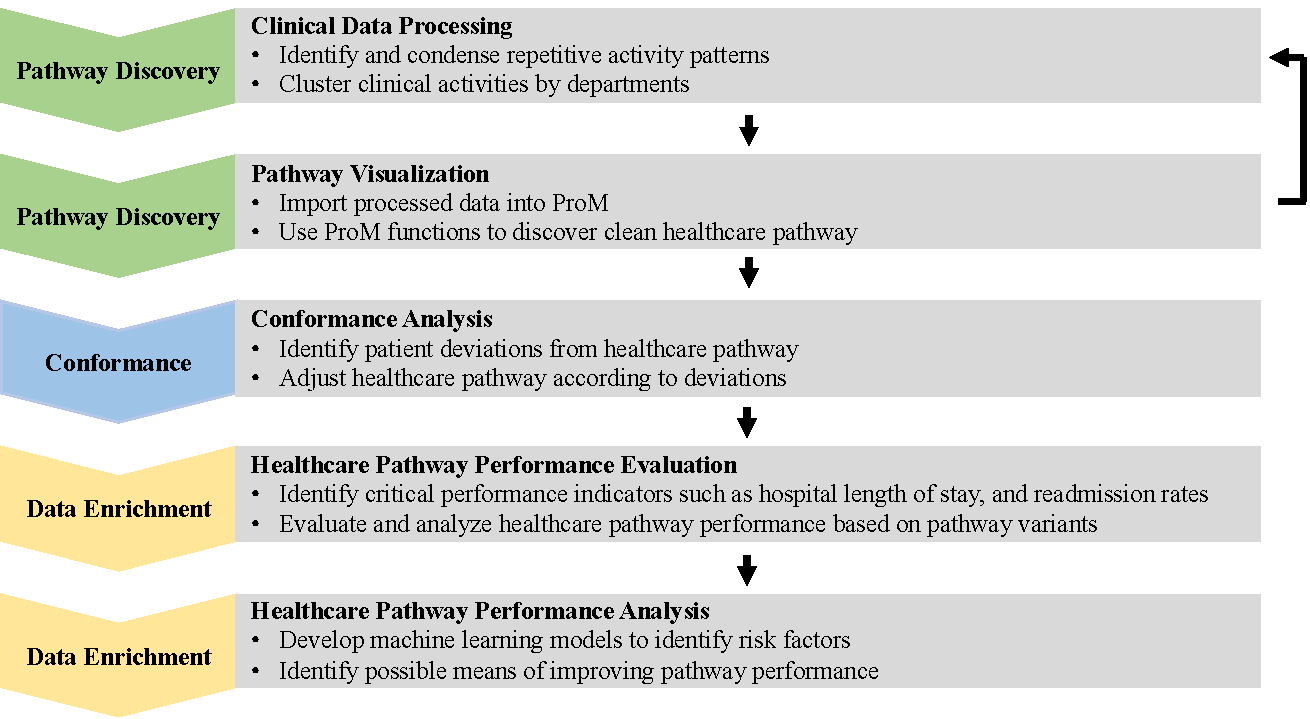
\includegraphics[width=\textwidth]{images/pipeline_diagram_journal.pdf}
\caption{The process mining pipeline comprises three sections, which
  are subdivided into five steps: Clinical data processing, pathway
  visualization, conformance analysis, healthcare pathway conformance
  evaluation, and predictive analytics of healthcare pathways. The
  first three steps are connected in two iterative cycles.}
\label{fig:pipeline}
\end{figure}

This study uses ProM (version 6.7) as the main process mining tool\footnote{\url{http://www.promtools.org}}. 
ProM is an open-source process mining software that is effective for construction of business models from input data files. ProM is chosen for this study because it has an intuitive user interface and supports many process mining plug-ins \cite{VanDongen2005}. The process mining and conformance analysis plug-ins supported by ProM are well documented. All these features of ProM make it easy for the process mining steps in the pipeline (see Fig.~\ref{fig:pipeline}) to be repeated by users with no background in process mining. The process mining techniques used in this paper are selected based on their ease for clinical interpretation and their potential to be combined with machine learning models. 

\subsection{Healthcare Pathway Discovery}
Healthcare pathway discovery is the first phase of the process mining pipeline. It consists of two steps: clinical data processing and pathway visualization, which are conducted iteratively until a concise model is produced.
The aim is to use patient healthcare records stored in hospital information systems to design a concise pathway model that is easy for clinical interpretation. Therefore, clinical input is critical to the selection of appropriate processing methods. 
 
Healthcare pathways generally have much higher levels of complexity than standard business processes, and unprocessed clinical data contains too many clinical variations for a clean and concise pathway model to be mined \cite{Huang2013, Veiga2010}. Each pathway variant is a unique event sequence of a complete patient trace. The ProM plug-in \plugin{Explore Event Log} (from the \texttt{Log Enhancement} package) extracts pathway variants from patient traces, and the total number of pathway variants is an indicator of the level of clinical variation between patient traces. The basic format of an example pathway variant extracted by \plugin{Explore Event Log} is demonstrated in  Fig.~\ref{fig:example pathway variant}.

\begin{figure}[t]
\centering

\includegraphics[width=\textwidth]{images/example_pathway_variant_format2.jpg}
\caption{
  Basic format of an example pathway variant visualized by
  ProM's plug-in \plugin{Explore Event Log}.
  The example process   consists of three different activities
  (colours).
  The start and stop event of each activity are indicated by a
  separate arrow, such that overlapping activities can be easily identified.}
\label{fig:example pathway variant}
\end{figure}

In order to reduce healthcare pathway variations to a meaningful pathway model, the pathway variants visualized by the plug-in \plugin{Explore Event Log} are examined closely to determine the most suitable processing methods. 
There are three effective methods for reducing clinical variations without filtering patient traces:

\begin{description}
    \item[Cluster clinical activities] that are similar in nature so that the range of activities is reduced to a manageable size, e.g., `Abdomen CT scan' and `Pelvis CT scan' could be clustered into a single activity under `CT scan'.
    \item[Merge consecutive clinical activities] that are performed consecutively into a single activity, e.g., a patient receiving the same medication five times on the same day could be regarded as a single activity.
    \item[Condense repetitive activity patterns] 
         that repeat but exhibit variable cycle length. These patterns indicate an activity that must be performed periodically while the patient is waiting for a different activity to begin, e.g., lab tests to monitor a patient’s condition, medication to prevent infection. These repetitive patterns could be condensed into a single, parallel activity.
\end{description}
Clinical input is highly recommended at this step particularly for complex or unfamiliar healthcare pathways. 

%\subsubsection{Pathway Visualization}

\subsection{Healthcare Pathway Conformance Analysis}
It is very difficult for clinicians to manually track individual patient traces through the treatment process and ensure that they are conforming to standard protocols. Identifying unwarranted deviations and making the required interventions early in the process has the potential to improve health outcomes and decrease cost. 
Conformance analysis identifies patient deviations by comparing the pathway model to clinical data. 
Accuracy of the discovered healthcare pathway model is validated if the majority of the patient traces conform to the model. Patient traces rarely all follow identical pathways, so the healthcare pathway model is not expected to capture all patient traces. The objective is to discover a healthcare pathway model that captures the fundamental structure of most patient traces and detect unexpected patient deviations. 

ProM offers tools for conformance analysis of healthcare
pathway models: Its plug-in \plugin{Inductive Visual Miner} compares
patient traces from input clinical data to a healthcare pathway model
and indicates patient traces which are deviating from the pathway
model.
For this purpose, the pathway model is visualized as a process tree,
which is a hierarchical map comprised of decision nodes and
tasks representing clinical activities
\cite{25a7fd818bf44606a903d9b78b95cdd3}.
Therefore, process trees enable the identification of pathway branches
throughout the healthcare pathway model (c.f. Sec~\ref{Sec:AppendicitisDiscoveryConformance}).

If valid patient traces deviate from a healthcare pathway model, 
adjustments are made to the model to improve patient conformance.
A typical example might be the introduction of a new form of
treatment, which has not been included into the model yet.
Including these findings into the model leads to an iterative approach
between pathway discovery and conformance analysis (Fig.~\ref{fig:pipeline}).
Conversely, conformance analysis can identify where invalid
patient traces deviate from the model and investigate the reason for
the discrepancy, e.g., clinicians following obsolete pathways or data errors.

\subsection{Healthcare Pathway Data Enrichment}
% \subsubsection{Healthcare Pathway Performance Evaluation}
Data enrichment of healthcare pathways is the third phase of the
discussed process mining pipeline (Fig.~\ref{fig:pipeline}).
It comprises two steps: Healthcare pathway performance evaluation and
healthcare pathway performance analysis.

The main objectives of evaluating healthcare pathway performance are
to understand the strengths and weaknesses of the current pathway design,
and to identify potential methods of improvement. Possible indicators
of healthcare pathway performance include waiting times of clinical
activities, hospital length of stay, recovery time, and readmission
rates \cite{Rotter2008_pathways}.
Most of these indicators can be calculated or estimated using standard clinical timestamps. Postoperative Length of Stay (PLS), which is measured from leaving operating theatre to discharge, can also be considered as patient recovery time.
For surgical healthcare pathways,  PLS is one of the critical indicators for evaluating healthcare pathway
performance \cite{Pearson2001_pathways}. 

Analysing the performance of healthcare pathways with respect to
pathway variants and other possible influencing factors like
demographics or patient specific pathway characteristics, e.g. surgery duration (SD), is the final step of the process mining pipeline
(Fig.~\ref{fig:pipeline}).
Due to the fact, that most pathway performance indicators do not
follow normal distributions, while exhibiting significant stochastic
volatility, neither classical hypotheses tests \cite{Goodman2008_p-value}, nor point-predicting
machine learning models are appropriate for analysing healthcare
pathways.
Instead, probabilistic machine learning models
\cite{Ghahramani2015_PML} are used for extracting interpretable models
from healthcare pathways (Sec.~\ref{sec:ML}).
For this purpose, feature engineering \cite{DongLiu2018_FE} from
the patients' pathway traces (e.g. SD, pathway variant),
demographics (e.g. age), as well as medical documentation like written
diagnosis, time series, or images become important.
In order to demonstrate this approach, the following case study
discusses a probabilistic machine learning model for PLS, which
takes into account pathway variants
(Sec.~\ref{Sec:AppendicitisDiscoveryConformance}), as well as demographics, and
SD (Sec.~\ref{sec:ML}).

\section{Case Study: Appendicitis Healthcare Pathways}
\label{Sec:Appendicitis}
This section discusses the healthcare pathway mining and analysis process for an appendicitis case study. For this purpose, two years’ worth of data
from 2015 to 2017 on 448 appendicitis patients have been analysed. This case study is selected because clinicians confirmed it is a relatively simple surgical pathway with clear start and end points.

\subsection{Data Description}
\label{Sec:DataDescription}
The patient records for this case study were collected from North
Shore Hospital in Auckland, New Zealand. The electronic patient
records in North Shore Hospital are stored using the Radiology
Information System (RIS) and the patient administration system iPM.
The extracted data were de-identified and an ethics approval for this research was obtained. All data sets collected from the hospital's information system on appendicitis patients are summarized in Tab.~\ref{table:data description table}. Theatre encounter is the system ID used to identify patient traces, and clinical activities are categorized by clinical departments (e.g. radiology, pharmacy). A column labelled `Pre-Op/Post-Op' indicates whether a clinical activity is performed before or after surgery, and contents of this column are appended as prefixes to the clinical activities during data processing. Processed data sets are imported into ProM for pathway discovery and conformance analysis.

\newcommand{\tabitem}{~~\llap{\textbullet}~~}

\begin{table}[t]
\centering
\caption{Description of all data sets collected from North Shore Hospital for the appendicitis case study.}
\label{table:data description table}
\begin{tabular}{lll}
  \hline
  \hline
EMR  &     Columns of Interest & Data Type  \\
\hline
Acute Theatre   &    \tabitem Theatre Encounter & String\\  &\tabitem Surgery Start Time & Datetime\\  &\tabitem Surgery End Time & Datetime\\  &\tabitem Into Theatre Time & Datetime\\  &\tabitem Out of Theatre Time & Datetime\\
  \hline
General Surgery   &    \tabitem Theatre Encounter & String\\  &\tabitem Admission Time & Datetime\\  &\tabitem Discharge Time & Datetime\\
  \hline
Radiology/Pharmacy  &    \tabitem Theatre Encounter & String\\ /Anesthesia   & \tabitem Clinical Activity & String\\  &\tabitem Clinical Activity Start Time  & Datetime\\  &\tabitem Pre-Op/Post-Op  & String\\
  \hline
Patient    &    \tabitem Theatre Encounter & String\\  &\tabitem Patient Age & Integer\\
  \hline
  \hline
\end{tabular}
\end{table}

\subsection{Appendicitis Pathway Discovery and Conformance Analysis}
\label{Sec:AppendicitisDiscoveryConformance}
The appendicitis pathway model, which has been generated by ProM's
plug-in \plugin{Explore Event Log}, is shown in
Fig.~\ref{fig:appendicitis pathway variants} in the form of a pathway
variant plot.
The pathway variants are extracted without activities related to medication (i.e. preoperative and postoperative cefuroxime/metronidazole) because the clinicians confirmed that antibiotics are usually taken while the patient is waiting for surgery or discharge. The duration of these activities are therefore highly variable and result in a high number of unique pathway variants.

%The variant specific numbers of patient traces given in  Fig.~\ref{fig:appendicitis pathway variants} are repeated in Tab.~\ref{table:appendicitis variant table}.
The pathway variant plot visualizes the 13 pathway variants of the
appendicitis model sorted from the most common pathway (index 0) to
the least common pathway (index 12).
The top four variants account for approximately 88\% of the patient
traces (Tab.~\ref{table:appendicitis variant table}).
All clinical activities are represented by a start event and a stop
event.
The activities are colour coded such that the same colour refers to the same clinical activity. The most common pathway variant (index 0) only consists of anesthesia and surgery, while the second most common variant (index 1) also includes preoperative X-ray.
The pathway variant indices are used in Sec.~\ref{sec:ML} as one-hot
encoded feature of the probabilistic machine learning model.

\begin{figure}[t]
\hspace{-2cm}
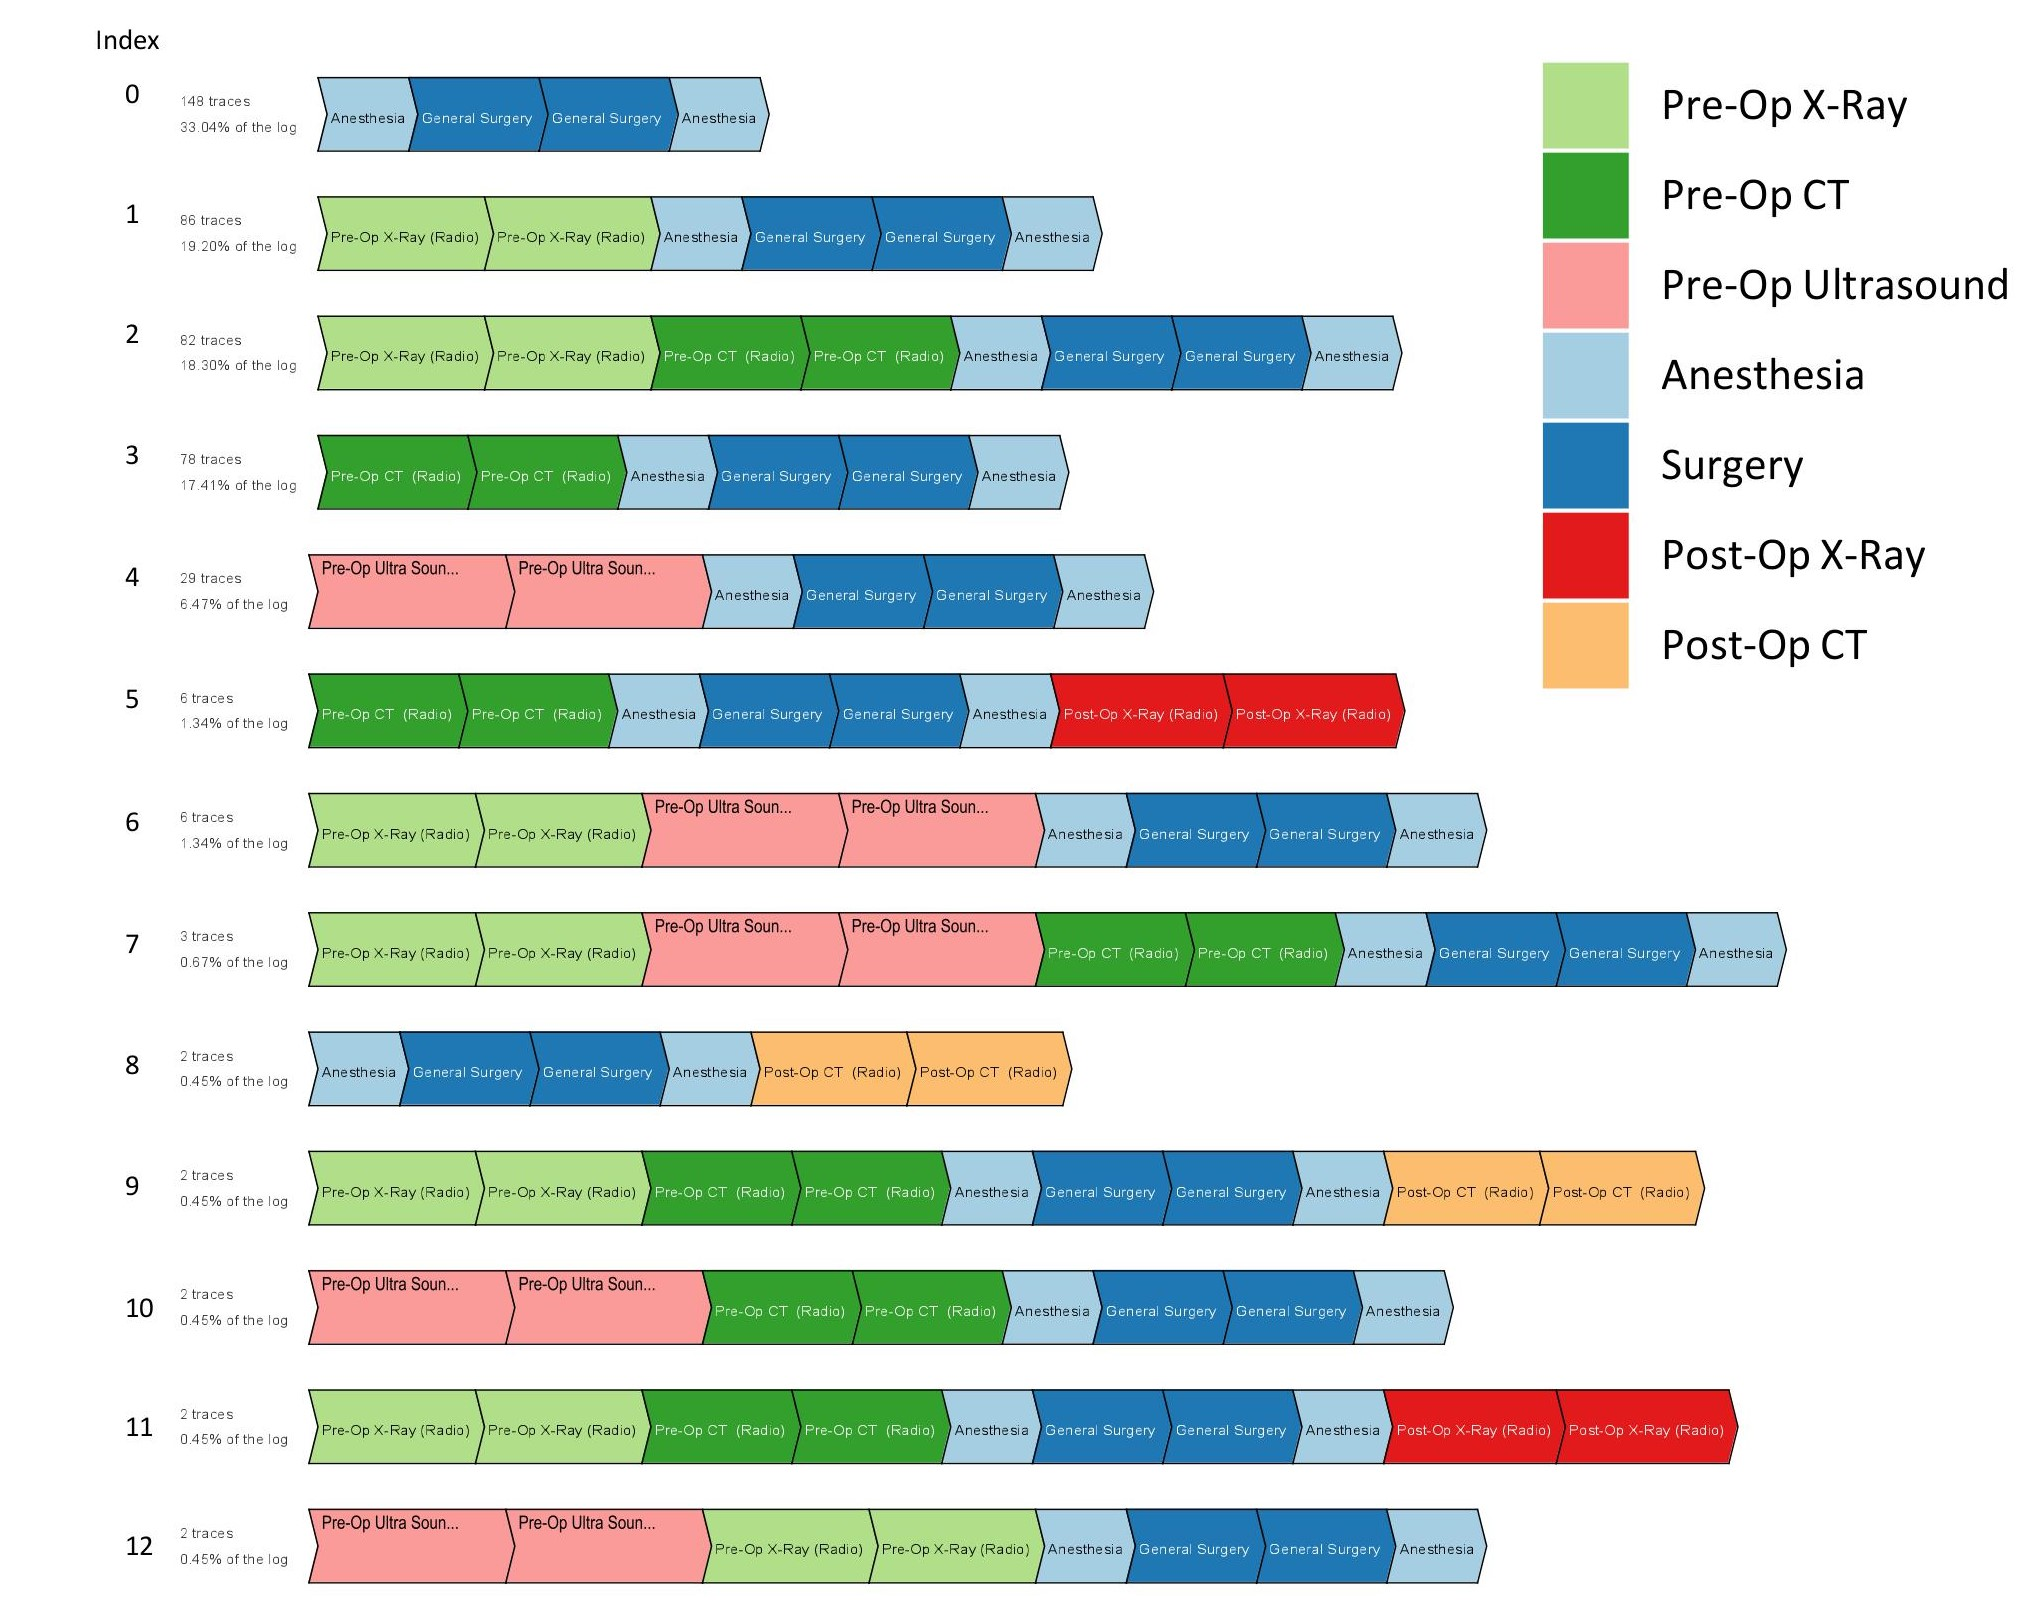
\includegraphics[width=1.5\textwidth]{images/appendicitis_variant_index_anes.jpg}
\caption{Appendicitis pathway variant plot auto-generated by ProM's
  plug-in \plugin{Explore Event Log}. 
  The plot visualizes the sequences of start and stop events for the different pathways.
  For the purpose of readability the legend was added and the
  statistics on the left are repeated in Tab.~\ref{table:appendicitis variant table}.
 The top four variants account for approximately 88\% of the patient
 traces. They are modelled as one-hot encoded features V0, V1, V2, and V3
 in Sec.~\ref{sec:ML}, while pathway variants V4--V12 together represent
 the base model.
 }
\label{fig:appendicitis pathway variants}
\end{figure}
\clearpage

\begin{table}[t]
\centering
\caption{Statistics of appendicitis patient traces shown in Fig.~\ref{fig:appendicitis pathway variants}.}
\label{table:appendicitis variant table}
\begin{tabular}{llllllll}
  \hline
  \hline
Variant &     0  &     1  &     2  &     3  &    4  &    5  &    6  \\
\hline
Patients   &    148 &     86 &     82 &     78 &    29 &     6 &     6 \\
  Percentage &  33.04\% &  19.20\% &  18.30\% &  17.41\% &  6.47\% &  1.34\% &  1.34\%\\
  \hline
  \hline
Variant &     7  &    8  &    9  &    10 &    11 &    12 \\
\hline
Patients   &   3 &     2 &     2 &     2 &     2 &     2 \\
Percentage &  0.67\% &  0.45\% &  0.45\% &  0.45\% &  0.45\% &  0.45\% \\
  \hline
  \hline
\end{tabular}
\end{table}

The first stage of the appendicitis pathway model visualized by \plugin{Inductive Visual Miner} is shown in Fig.~\ref{fig:ivm pathway model example}.
Unlike the pathway variants, this appendicitis pathway model incorporates activities representing antibiotics. The model indicates that 42 patients perform ultrasound and 183 patients perform X-ray upon admission. 

\begin{figure}[t]
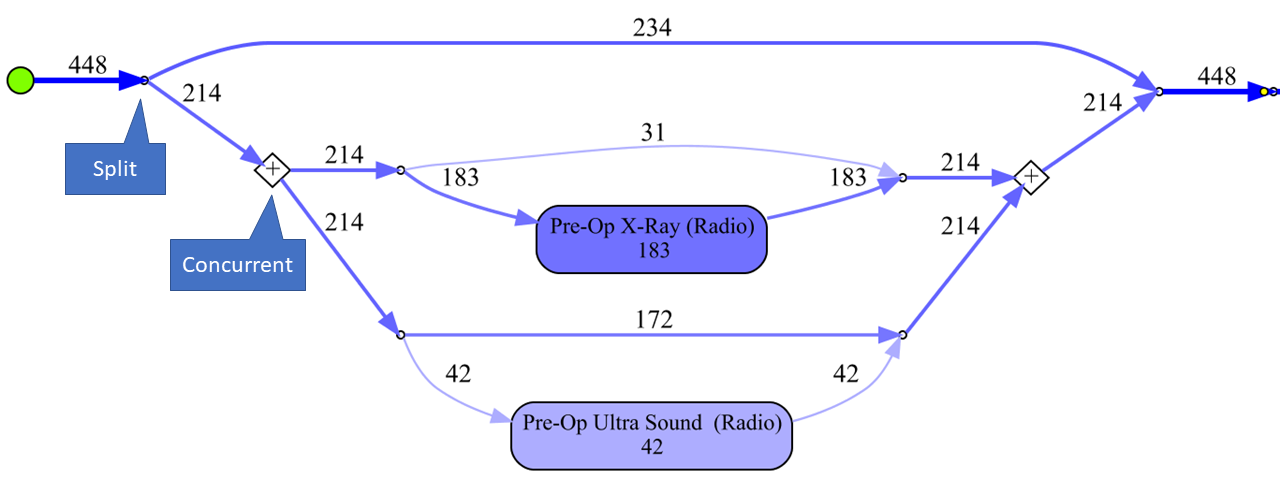
\includegraphics[width=\textwidth]{images/ivm_appendicitis_first_stage_example.png}
\caption{First stage of the appendicitis pathway model generated by
  ProM. The following stages have been omitted for the purpose of
  readability.
  The process indicates that 234 patients do not have any preoperative
  imaging diagnostics, while 214 patients enter the imaging
  diagnostics branch.
  Please refer to Leeman's manual on \plugin{Inductive Visual Miner} for details on the model notations \cite{leemansinductive}.}
\label{fig:ivm pathway model example}

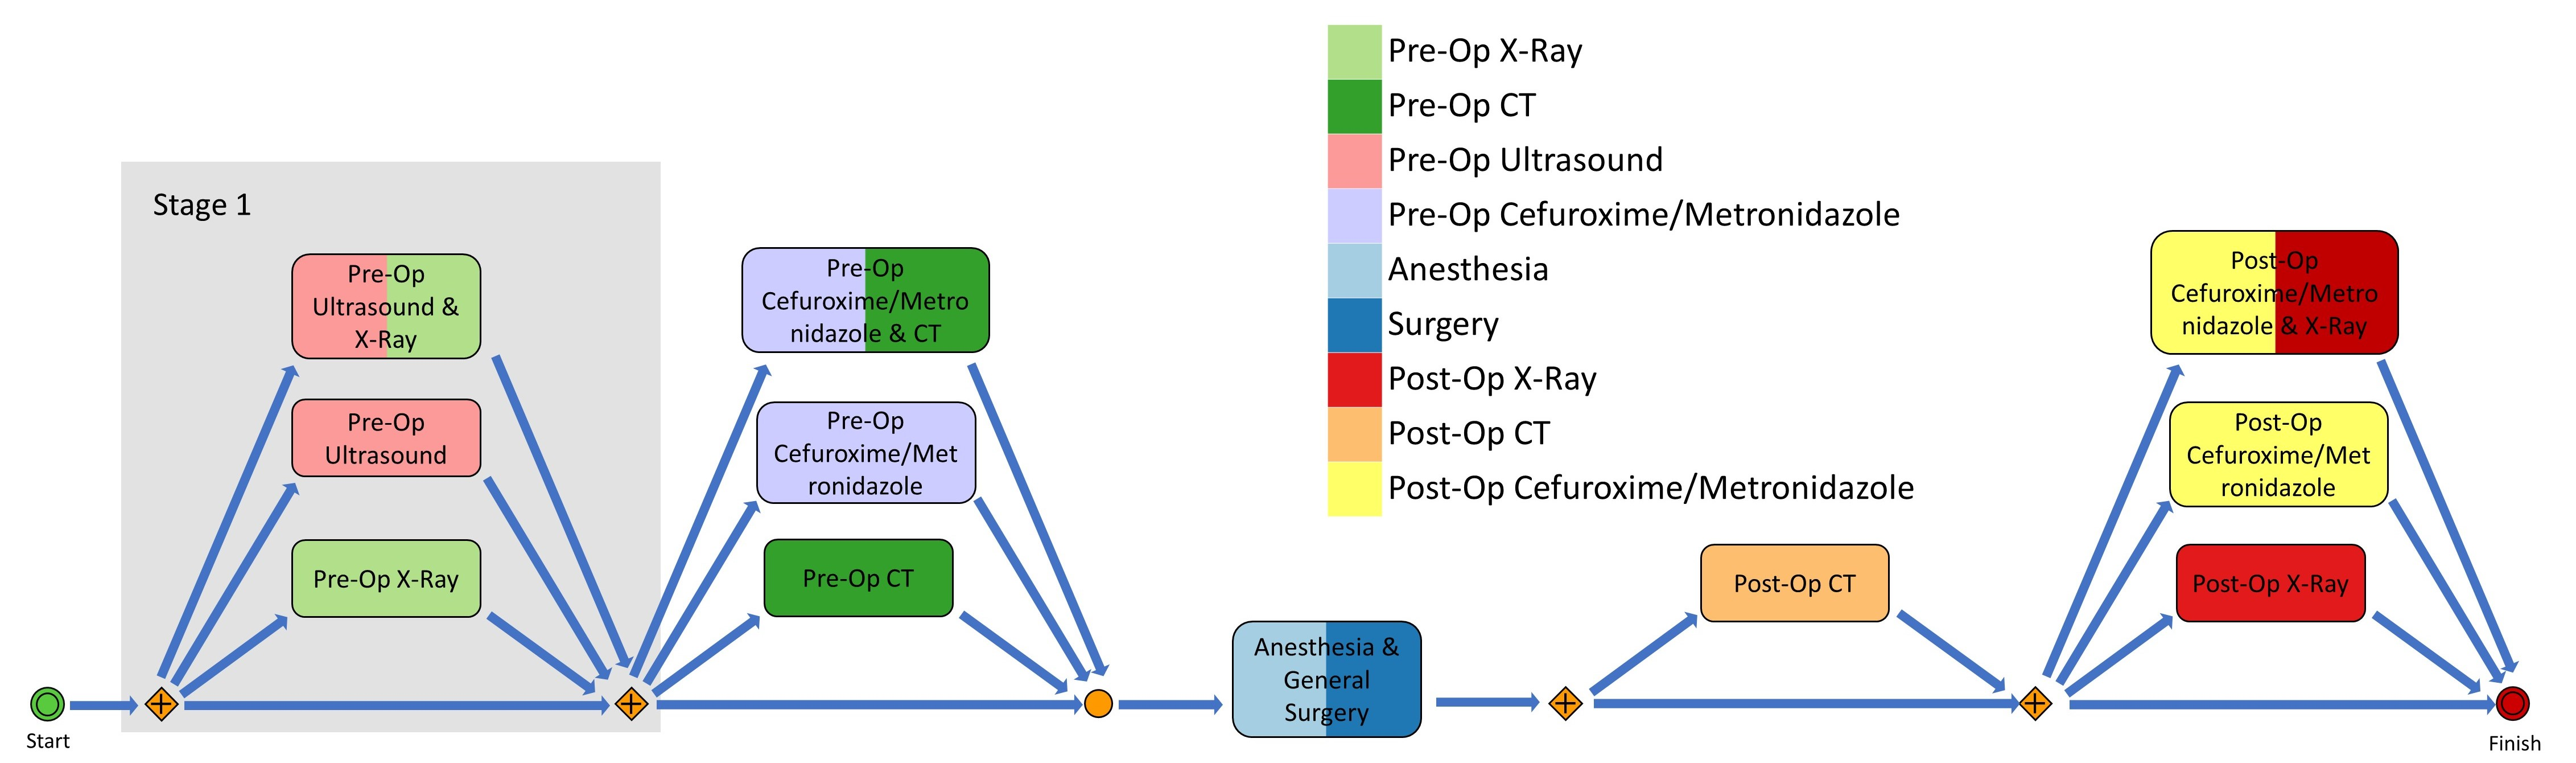
\includegraphics[width=\textwidth]{images/communicative_appendicitis_process_models_anes.jpg}
\caption{Appendicitis pathway model using nomenclature of Tab.~\ref{table:notation table}. All preoperative and
  postoperative activities belong to radiology and pharmacy
  departments. Preoperative antibiotics are taken in the second stage
  of the treatment pathway.}
\label{fig:appendicitis pathway model}
\end{figure}

While the complex process tree notation of ProM's \plugin{Inductive
  Visual Miner} plug-in is optimal for detailed analysis, it has been
reformulated under new notations for easy clinical interpretation.
The new model notations are summarized in Table \ref{table:notation
  table}, and the reformulated appendicitis pathway model is shown in
Fig.~\ref{fig:appendicitis pathway model}. The section of the model
labelled as `Stage 1' in Fig.~\ref{fig:appendicitis pathway model}
corresponds to the process tree shown in Fig.~\ref{fig:ivm pathway
  model example}.
This is the final pathway model that has been compiled based on
clinical input to account for valid patient deviations, and all
patient traces conform to the updated pathway.
The most common pathway variant (index 0) shown in Fig.~\ref{fig:appendicitis pathway variants} corresponds to the horizontal path from start to finish in Fig.~\ref{fig:appendicitis pathway model}.
Feedback from medical experts confirmed that the simplified
appendicitis pathway model (Fig.~\ref{fig:appendicitis pathway model})
correctly represents the As-Is process, while being easily
interpretable.

\begin{table}[t]
\centering
\caption{Definitions of new pathway model notations.}
\label{table:notation table}
\begin{tabular}{ l c l }
 \hline
 \hline
 Notation & Symbol & Definition \\ 
 \hline
 Orange Diamond 
 &
%\raisebox{-\totalheight}{\includegraphics[width=0.3\textwidth, height=60mm]{images/myLboro.png}}
 \raisebox{-3pt}{
\includegraphics[width=0.5cm]{images/decision_node.png}}
 & Decision Point, indicating exclusive choice \\ 
 \hline
 Orange Connector 
 & 
 \raisebox{-3pt}{
\includegraphics[width=0.5cm]{images/connection_node.png}}
 & Pathway Connection Point \\
 \hline
 Green Connector 
 & 
 \raisebox{-3pt}{
\includegraphics[width=0.5cm]{images/start_node.png}}
 & Starting Point \\
 \hline
 Red Connector 
 & 
 \raisebox{-3pt}{
\includegraphics[width=0.5cm]{images/finish_node.png}} 
 & Finishing Point \\
 \hline
 \hline
\end{tabular}
\end{table}

\subsection{Length of Stays of Appendicitis Pathway Variants}
Length of stays in hospital are analyzed based on the 13 identified
appendicitis pathway variants shown in Fig.~\ref{fig:appendicitis
  pathway variants}. Postoperative length of stay, measured from
leaving theatre to discharge, for each of the 13 appendicitis pathway
variants are shown in Fig.~\ref{fig:post op length of stay
  appendicitis}. Pathway variant 9 has the longest postoperative
length of stay. Pathway variants 5, 7 and 11 also have relatively long
postoperative length of stays.
Only pathway variant 7 does not include any postoperative activities.
The number of patient traces that follow each pathway variant is limited, and more samples are required to identify rate-determining steps. Probabilistic machine learning models are used to further investigate factors influencing postoperative length of stay (Sec.~\ref{sec:ML}).

\begin{figure}[t]
\centering
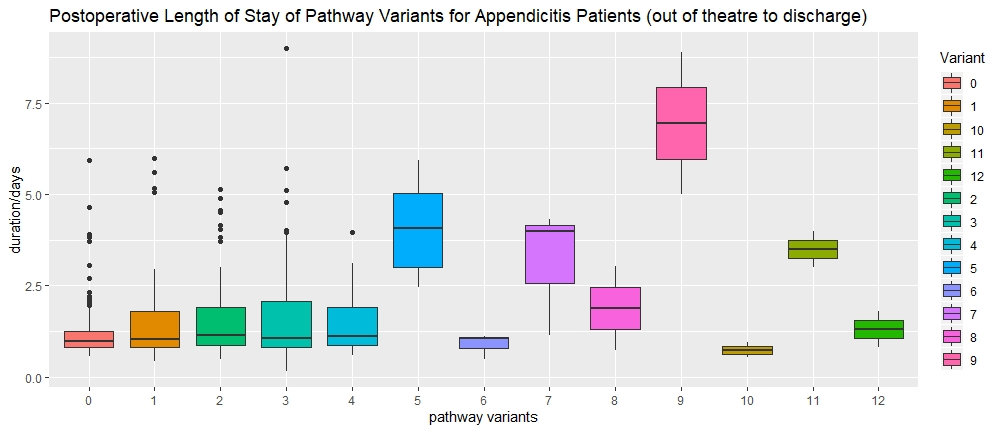
\includegraphics[width=\textwidth]{images/postoperative_length_of_stay_appendicitis.jpeg}
\caption{Postoperative length of stay of the 13 appendicitis pathway variants, measured from leaving theatre to discharge.}
\label{fig:post op length of stay appendicitis}
\end{figure}

\section{Probabilistic Machine Learning Model for Postoperative Length of Stay of Appendicitis Patients}
\label{sec:ML}
The following section investigates the question of whether the pathway
variants of the appendicitis case study are relevant features or
covariates for explaining the stochastic volatility of postoperative
Length of Stay (PLS, Fig.~\ref{fig:Geom}a), which is measured from
leaving operating theatre to discharge.
This is quite a challenging task, because the individual healing process is expected to depend on personal factors like age \cite{polanczyk2001impact} as well as the individual severity of the appendicitis inflammation, which in general is unknown at this stage of the data analysis, but might be captured by proxies like surgery duration (SD). 

\begin{figure}
  \centering
  \begin{tabular}{ll}
    (a) & (b) \\
    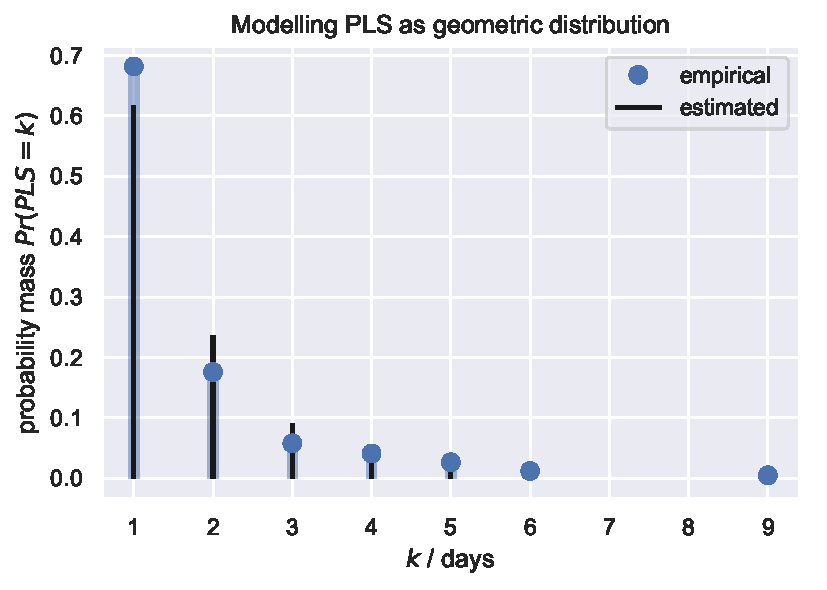
\includegraphics[width=0.5\textwidth]{images/DS19eH1_G0__empirical_geometric.pdf}
    &
    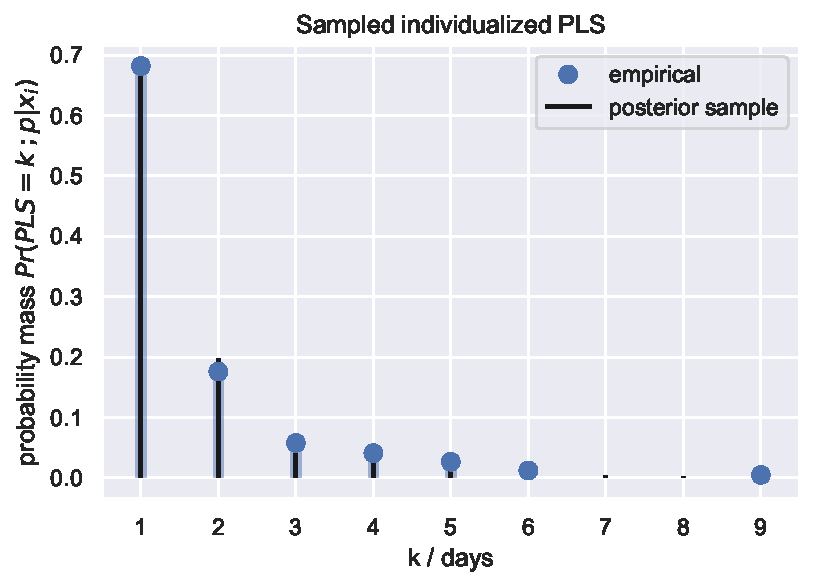
\includegraphics[width=0.5\textwidth]{images/DS19fk1_c0__sampled_posterior.pdf}\\
  \end{tabular}
    \caption{Modelling PLS as geometric distribution without patient
      specific model (a) and with individualised posterior (b) from
      model B (Eq. \eqref{modelB}). Sampling from patient specific
      posterior distributions replicates the observed PLS quite well.
      }
    \label{fig:Geom}
\end{figure}

For the purpose of this analysis, patients' traces with complete
demographic information (415 samples) are selected and
the patients' $PLS$, which is
calculated as the time interval between leaving operating theatre and discharge, is
converted into the number of days after surgery. Therefore, a $PLS$ of
one corresponds to a patient who has been discharged the day after
surgery. Three of the $N=415$  %DS19fA0
patient traces had a PLS of zero, because the surgery ended shortly after midnight and the patients were discharged on the same day. In order to simplify our analysis, the interpretation of PLS was broadened to the number of night rests after surgery, such that the PLS of these three patients could be projected to one.

Analysing the PLS of the 415 appendicitis patients reveals a
histogram which closely resembles a Geometric distribution (Fig.~\ref{fig:Geom}a)
\begin{equation}
Pr(PLS=k) = \text{Geom}(k; p) = (1-p)^{k-1}p^{k},
\end{equation}
parameterized by probability $p$ of being discharged on the $k^\text{th}$ day, respectively $k$ nights of rest after surgery. 
However, estimating $p$ as inverse mean of the observed PLS to 
\begin{equation}
 \hat{p} = \frac{N}{\sum\limits_{i=1}^N PLS_i} \approx 61.8\%	
\end{equation}
reveals that the average discharge probability $\hat{p}$ does not
generalize well over the cohort (Fig.~\ref{fig:Geom}a), because the number of patients being discharged on the first day after surgery is underestimated and the number of patients being discharged on the second and third day after surgery is overestimated.

For the following probabilistic machine learning models, the individualized discharge probability $p_i$ is modelled as a generalized linear model (GLM) using the inverse logistic function (logit) as a link function and the geometric distribution for generating the likelihood. 
For the following analysis, we are comparing two different models of
discharge probability $p_i$ as
\begin{equation}\label{modelA}
  \begin{split}
  \text{logit}(p_i) \sim & \;SD_i + \text{log}(age_i) + 
                            V_{0,i} + V_{1,i} + V_{2,i} + V_{3,i} + V_{0,i}\times\text{log}(age_i) +\\
  &   V_{1,i}\times\text{log}(age_i) + V_{2,i}\times\text{log}(age_i) + V_{3,i}\times\text{log}(age_i),\\
  \end{split}
\end{equation}
which we refer to as \textit{model A}, and
\begin{equation}\label{modelB}
  \begin{split}
  \text{logit}(p_i) \sim & \;SD_i + \text{log}(age_i) +
                                                         V_{0,i} + V_{1,i} + V_{2,i} + V_{3,i} + V_{0,i}\times\text{log}(age_i) +\\
  &    V_{1,i}\times\text{log}(age_i),\\
  \end{split}
\end{equation}
which we refer to as \textit{model B}.
These two models have been selected because they were the most
credible based on the widely applicable information criterion
(WAIC) and leave-one-out cross-validation (LOO) statistics
\cite{Vehtari2017_WAIC_LOO}.
The explanatory variables $V_{j,i}$ are categorical with 
\begin{equation}
V_{j,i} = \begin{cases}
	1: & V_{j,i} = j,\\
        0: & \text{otherwise}.
\end{cases}
\end{equation}
Therefore, the case $V_{0,i}=V_{1,i}=V_{2,i}=V_{3,i}=0$ corresponds to variants V4--V12 of Fig.~\ref{fig:appendicitis pathway variants}.
Models A and B make the simplifying assumption that the individualised
probability of discharge $Pr(PLS_i=k|x_i)$ can be estimated from 
\begin{equation}
x_i = (SD_i, \text{log}(age_i), V_{0,i}, V_{1, i}, V_{2, i}, V_{3, i}).
\end{equation}
 being available at the end of surgery, when future treatment steps and therefore the complete pathway variant for the respective $i^\text{th}$ patient have been decided on:
\begin{equation}
\begin{split}
Pr(PLS_i=k|x_i) & = \text{Geom}\left(k;p(x_i)\right) \\
& = \left(1-p(x_i)\right)^{k-1}\left(p(x_i)\right)^{k} \\
%& = \left(1-\mathbb{E}_{x_i}[p]\right)^{k-1}\left(\mathbb{E}_{x_i}[p]\right)^{k} \\
          %        & = \left(1-\text{logistic}(f(x_i))\right)^{k-1}\text{logistic}(f(x_i))^{k} \\
          %        & = \left(1+e^{f(x_i)}\right) \left(2 + e^{-f(x_i)} + e^{f(x_i)}\right)^{-k}
\end{split}
\end{equation}
with $p(x_i)$ being modelled either by Eq. \eqref{modelA} or
\eqref{modelB}.
    
The statistical model has been fitted using PyMC3
\citep{Salvatier2016_PyMC3} version 0.24.2 using the No-U-Turn Sampler
(NUTS) with 20,000 samples, 2,000 tuning steps, 2 chains, and an
acceptance rate of 90\%. The 95\% credible intervals of the estimated
model coefficients are shown in Fig.~\ref{fig:forest_plots}. The
Gelman-Rubin convergence statistic Rhat is close to one for all
coefficients (Tab.~\ref{tab:coeff}). 
However, for Model A the coefficients of the interaction terms
$\text{log}(age_i)\times V_2$ and $\text{log}(age_i)\times V_3$ are
close to zero with negative expectation values but a 25\% and 15\%
probability of being larger than zero (Tab.~\ref{tab:coeff}). 
Therefore, we have decided to focus the following analysis of the
fitted model on Eq.~\eqref{modelB} for which all credible intervals
exclude zero (Fig.~\ref{fig:forest_plots}b).
However, this does not change the overall trend depicted in Fig.~\ref{fig:posterior}.
It is important to note that both the coefficients of $SD$ and $\text{log}(age)$ are negative. This means that for the base model of variants V4--V12 as well as variants V2 and V3, the probability of discharge decreases with increasing SD and age. 
Compared to the base model, Variants V2 and V3 have a higher discharge probability because both coefficients are positive. 
The situation is more complicated for variants V0 and V1, because their coefficients are negative but the coefficients of their interaction terms with $\text{log}(age)$ are positive, which basically counterbalances the effect of $\text{log}(age)$.

\begin{figure}
  \centering
    \begin{tabular}{ll}
(a) Model A \eqref{modelA} & (b) Model B \eqref{modelB}\\
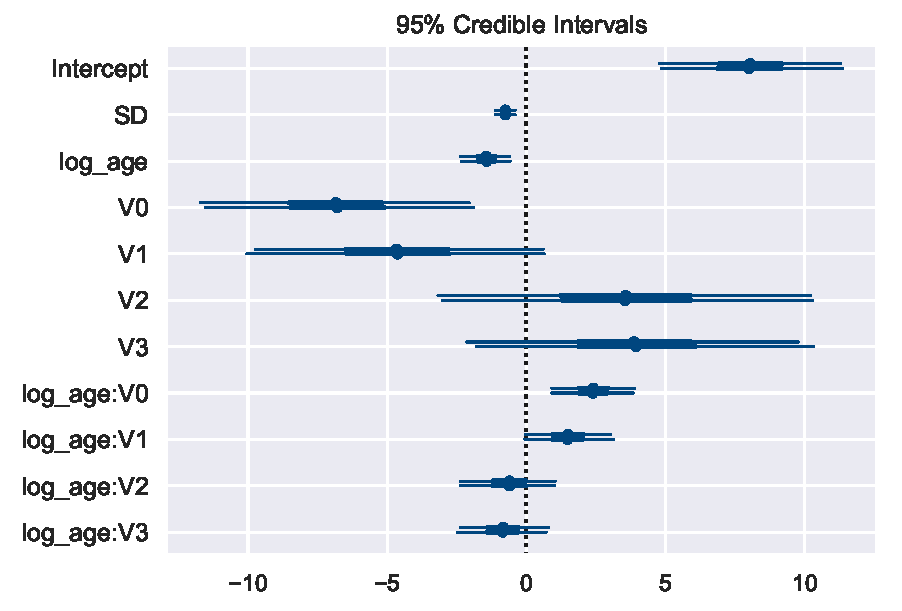
\includegraphics[width=0.5\textwidth]{images/DS19fm0_c0__forestplot_model_A.pdf}&
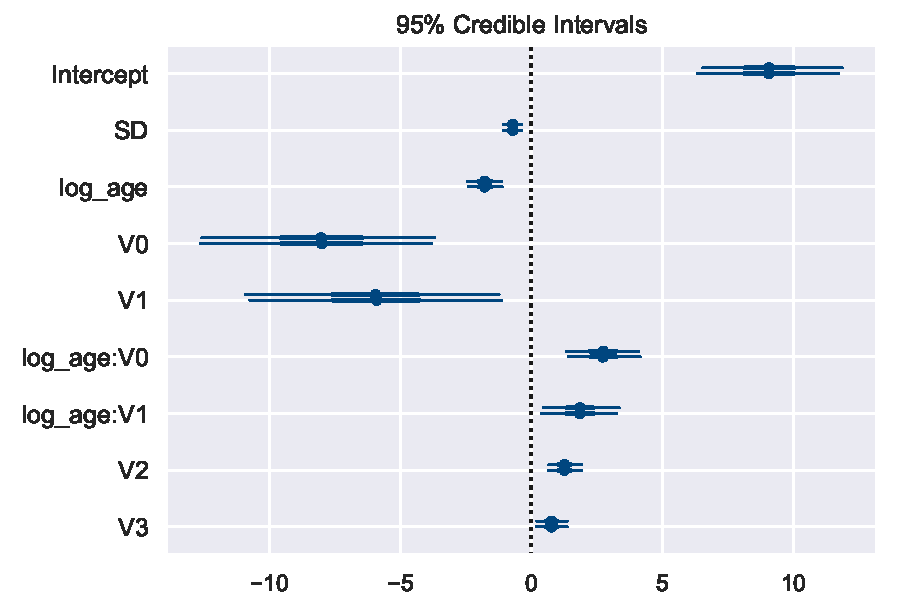
\includegraphics[width=0.5\textwidth]{images/DS19fk1_c0__forestplot_model_B}\\
\end{tabular}
    \caption{Credible intervals for models A \eqref{modelA} and B \eqref{modelB}.}
    \label{fig:forest_plots}
\end{figure}

\begin{table}
\caption{\label{tab:coeff} Coefficients of model B. Rhat is the
  potential scale reduction factor. A value of one indicates
  convergence.}
\centering
\begin{tabular}{lrrrr}
\hline
\hline
{} &      mean &    hpd\_2.5 &   hpd\_97.5 &      Rhat \\
\hline
Intercept  &  9.09 &   6.48 &  11.85 &  0.999988 \\
SD        & -0.71 &  -1.059 &  -0.371 &  0.999987 \\
log\_age    & -1.781 &  -2.46 &  -1.154 &  0.999988 \\
V0         & -8.04 & -12.56 &  -3.70 &  0.999980 \\
V1         & -5.95 & -10.82 &  -1.186 &  1.000013 \\
log\_age:V0 &  2.75 &   1.365 &   4.12 &  0.999980 \\
log\_age:V1 &  1.864 &   0.423 &   3.32 &  1.000013 \\
V2         &  1.267 &   0.646 &   1.901 &  1.000062 \\
V3         &  0.766 &   0.199 &   1.363 &  1.000046 \\
\hline
\hline
\end{tabular}
\end{table}


\begin{figure}
    \centering
    \begin{tabular}{ll}
(a)  & (b) \\
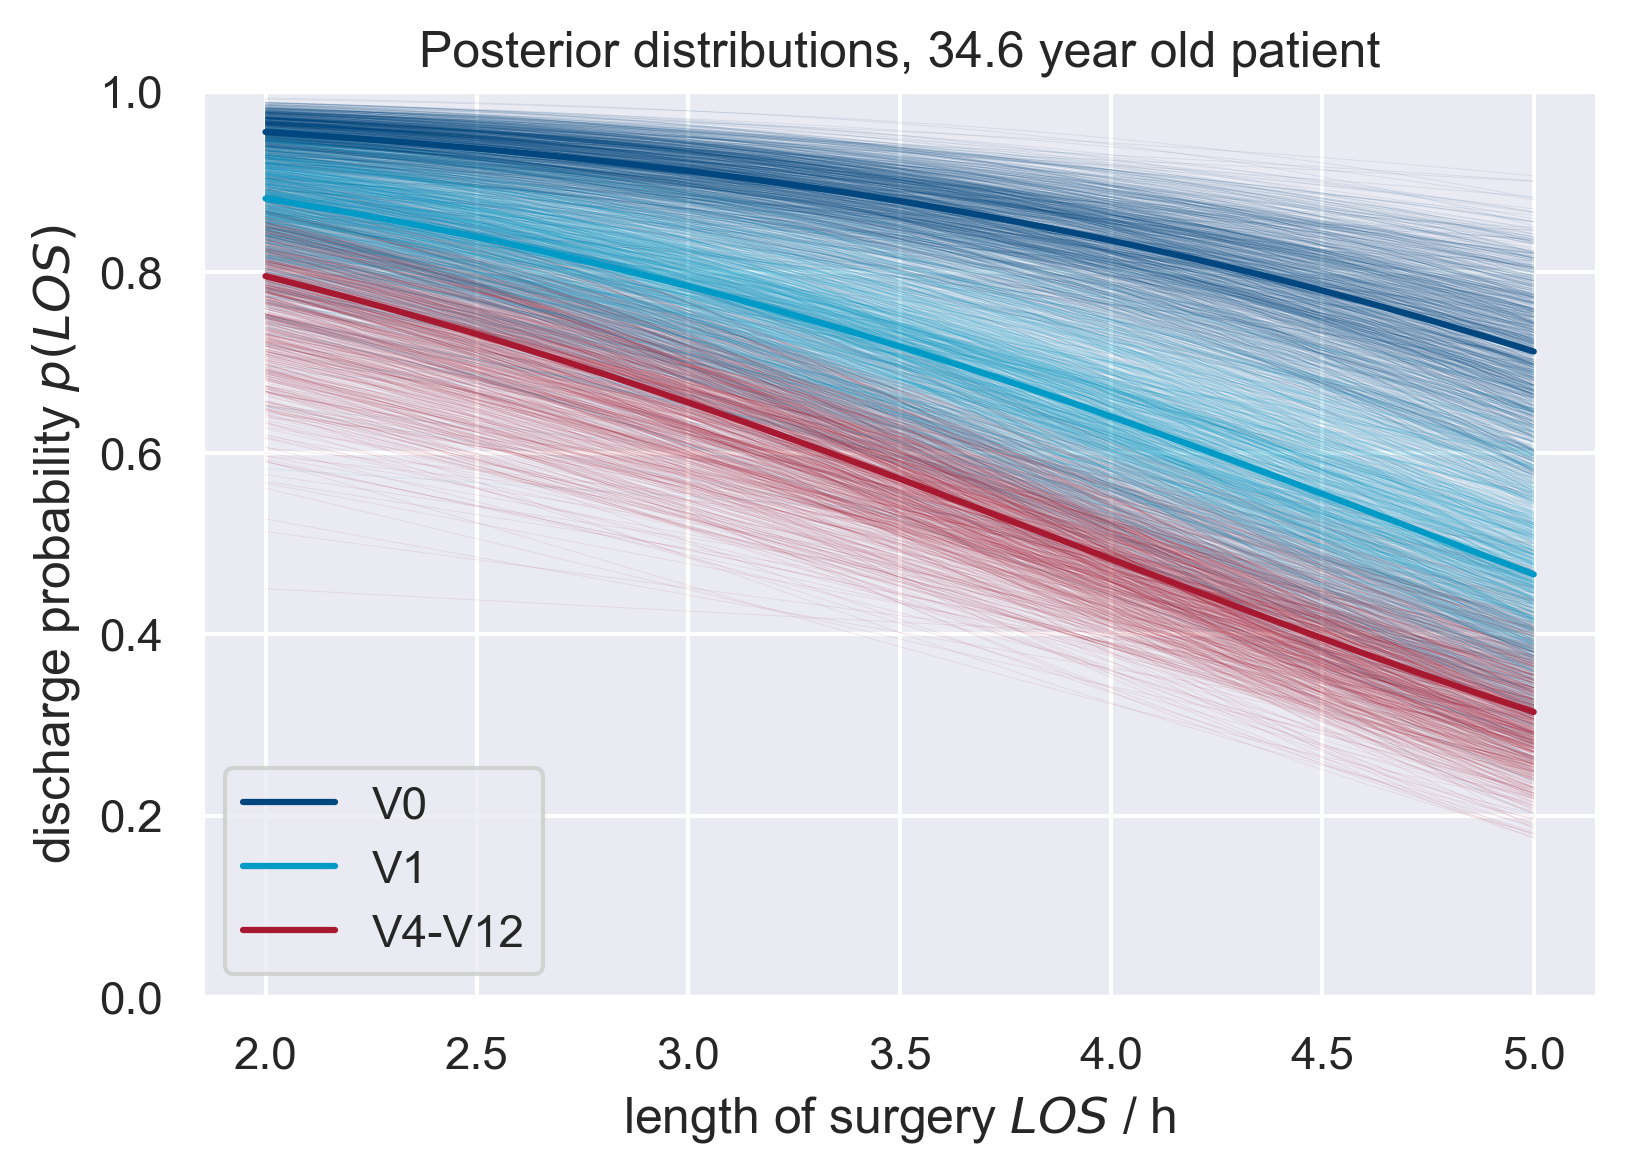
\includegraphics[width=0.5\textwidth]{images/DS19fk1_c0__p_LoS__model_B__traces_V0_V4-12__age_mean.png}&
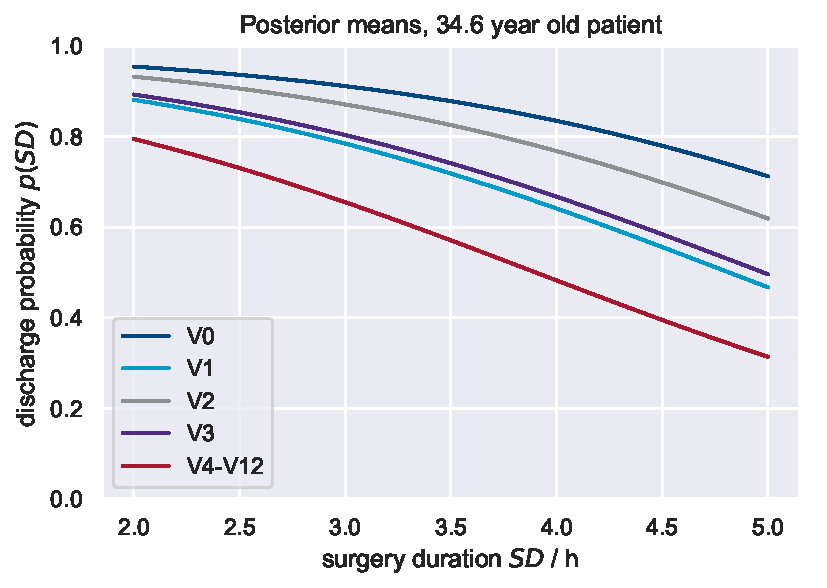
\includegraphics[width=0.5\textwidth]{images/DS19fk1_c0__p_LoS__model_B__mean__age_mean.pdf}\\
(c) & (d) \\
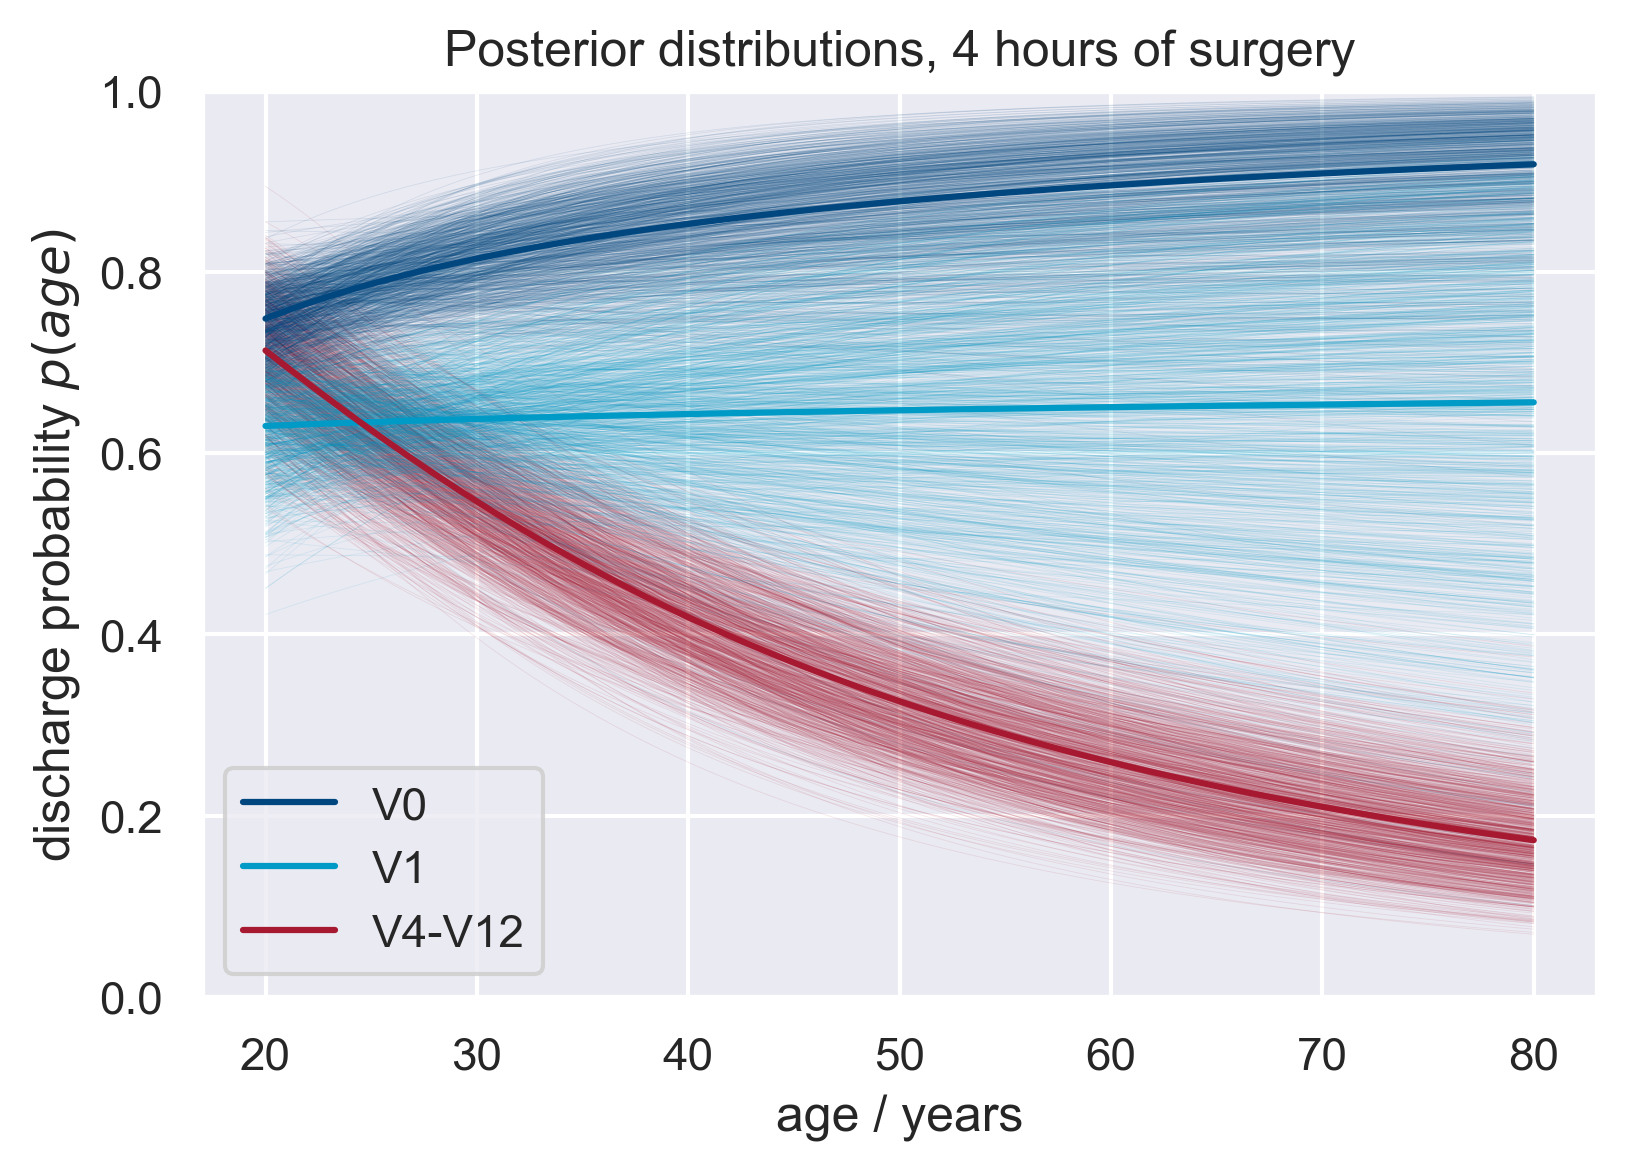
\includegraphics[width=0.5\textwidth]{images/DS19fk1_c0__p_age__model_B__traces__LoS_4h.png}&
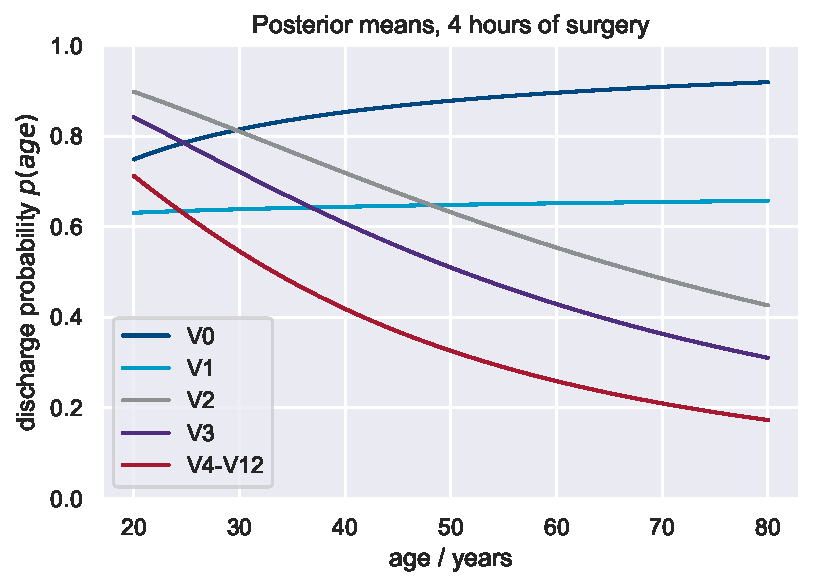
\includegraphics[width=0.5\textwidth]{images/DS19fk1_c0__p_age__model_B__mean__LoS_4h.pdf}\\
\end{tabular}
    \caption{Posterior distributions and corresponding means for
      different pathway variants of model B \eqref{modelB}. Trends with respect to
      SD and age are similar for model A \eqref{modelB}.}
    \label{fig:posterior}
\end{figure}

This is visualized in Fig.~\ref{fig:posterior}, which shows the posterior distributions of discharge probability $p_i$ as function of SD (Fig.~\ref{fig:posterior}a) and age (Fig.~\ref{fig:posterior}c). While the discharge probability decreases with increasing SD for all pathway variants (Fig.~\ref{fig:posterior}b), the effect is different for age. 
The discharge probability $p_i$ decreases for Variants V2, V3, and V4-V12 with increasing age of the patients, while its expectation value is constant for $V1$ and even increases by nearly 10\% for V0. Note, that the corresponding graphics for model A \eqref{modelA}, which are not shown here, resemble nearly the same correlations. 
From the clinical perspective, the difference in effects of age with
respect to the pathway variants might be related to the fact that the
most common pathway variants V0 and V1 are predominantly followed by younger patients (Fig.~\ref{Fig:boxplot}) and possibly older patients, for whom no complications are expected. 
However, the uncertainty of discharge probabilities for V1 is significantly larger compared to V0.

\begin{figure}
  \centering
  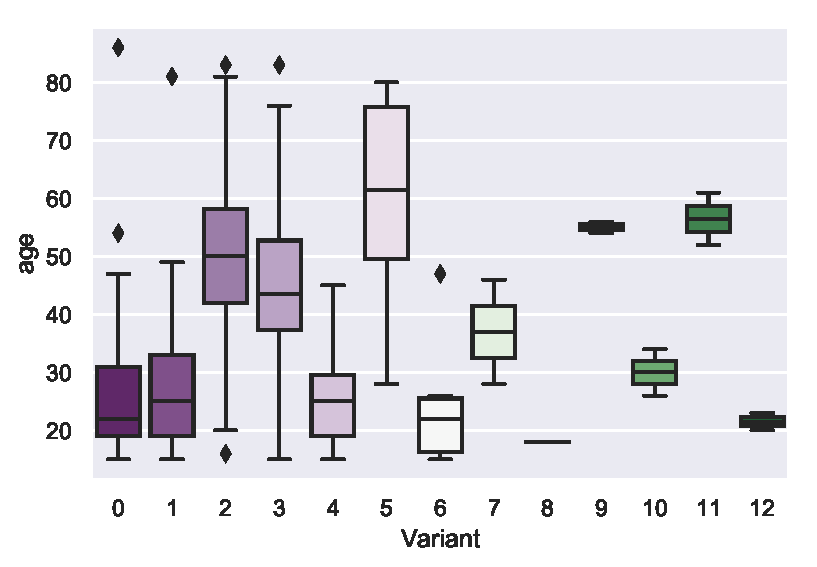
\includegraphics[width=0.618\textwidth]{images/DS19fA0_Lin20180730a__boxplot_age_variant.pdf}
\caption{Boxplot of patients' age for pathway variants of the
  appendicitis model.}
\label{Fig:boxplot}
\end{figure}

\section{Conclusion and Outlook}
\label{Sec:Conclusion}
Healthcare pathways are critical for maintaining quality of care and
improving health outcome for all patients, but there is no consensus
on a healthcare pathway mining pipeline suitable for hospital
implementation that supports pathway discovery from hospital health
records.
Business process modelling methods are used to design a process mining
pipeline that produces concise and comprehensible healthcare pathway
models from hospital records, and supports conformance analysis and
enrichment of the discovered pathways.
The proposed process mining pipeline successfully constructs concise
pathway models for the appendicitis case study.
The produced healthcare pathway models are easy for clinical
interpretation and provide an unbiased overview of real patient traces
through the treatment process.
Probabilistic machine learning models for predicting postoperative
length of stay, using information extracted by the process mining
pipeline, is showing promising results.
This means that the proposed mining pipeline has the potential to
support the development of machine learning models to further relate
healthcare pathways to performance indicators.
This study has established the use of business process modelling methods for the improvement of healthcare pathway mining methods, and there is value in investigating the capabilities of other business process modelling tools for healthcare pathway mining purposes.

\begin{table}[h]
\centering
\begin{tabular}{p{11cm}} 
 Summary points\\ 
 What was already known:
 \begin{itemize}
     \item Healthcare pathways are critical for reducing clinical variability, affecting operational excellence, and thereby maximizing health outcomes.
     \item  Most healthcare pathways result from clinician-led practice rather than explicit pathway design via a consensus model and systems approach. 
     \item  There is currently no consensus on a systematic healthcare pathway mining method that supports explicit design and conformance analysis of concise and comprehensible healthcare pathway models.
 \end{itemize}
 What this study adds:
 \begin{itemize}
     \item  The use of business process modelling methods improves the automatic mapping of healthcare pathways from electronic patient records.
     \item The application of business process modelling methods to
       healthcare pathway enables deviations from typical treatment
       pathways to be identified, all using standard clinical data
       timestamps.
     \item Probabilistic machine learning models enable the prediction
       of patient specific discharge probabilities, which lead to
       patient specific postoperative
       length of stay distributions.
 \end{itemize}
\end{tabular}
\end{table}
